\subsection{Sprint 6: da 2024-06-15 a 2024-06-24}
\par Con l'avvenuta integrazione dei nuovi \glossario{framework}, il team si presta a realizzare pagine e componenti essenziali dell'applicazione; questi sforzi mirano a migliorare l'interfaccia grafica e le funzionalità del prodotto.


\subsubsection{Obiettivi}
\begin{itemize}
  \item Miglioramento della struttura dei casi d'uso nell'\AdR;
  \item Revisione dei grafici nell'\AdR;
  \item Revisione dei requisiti funzionali;
  \item Ampliamento dei casi d'uso con la gestione del \glossario{debug} e degli errori;
  \item Aggiornamento del \PdP\ (stesura delle sezioni incomplete e revisione dei consuntivi precedenti);
  \item Stesura della dashboard di valutazione della qualità nel \PdQ;
  \item Inserimento dei grafici nel \PdQ;
  \item Stesura dei verbali interni ed esterni;
  \item Creazione componente di login funzionante;
  \item Sviluppo delle pagine \glossario{front-end} (chat, gestione dei \glossario{dizionari dati} e debug).
\end{itemize}

\begin{figure}[H]
  \centering
  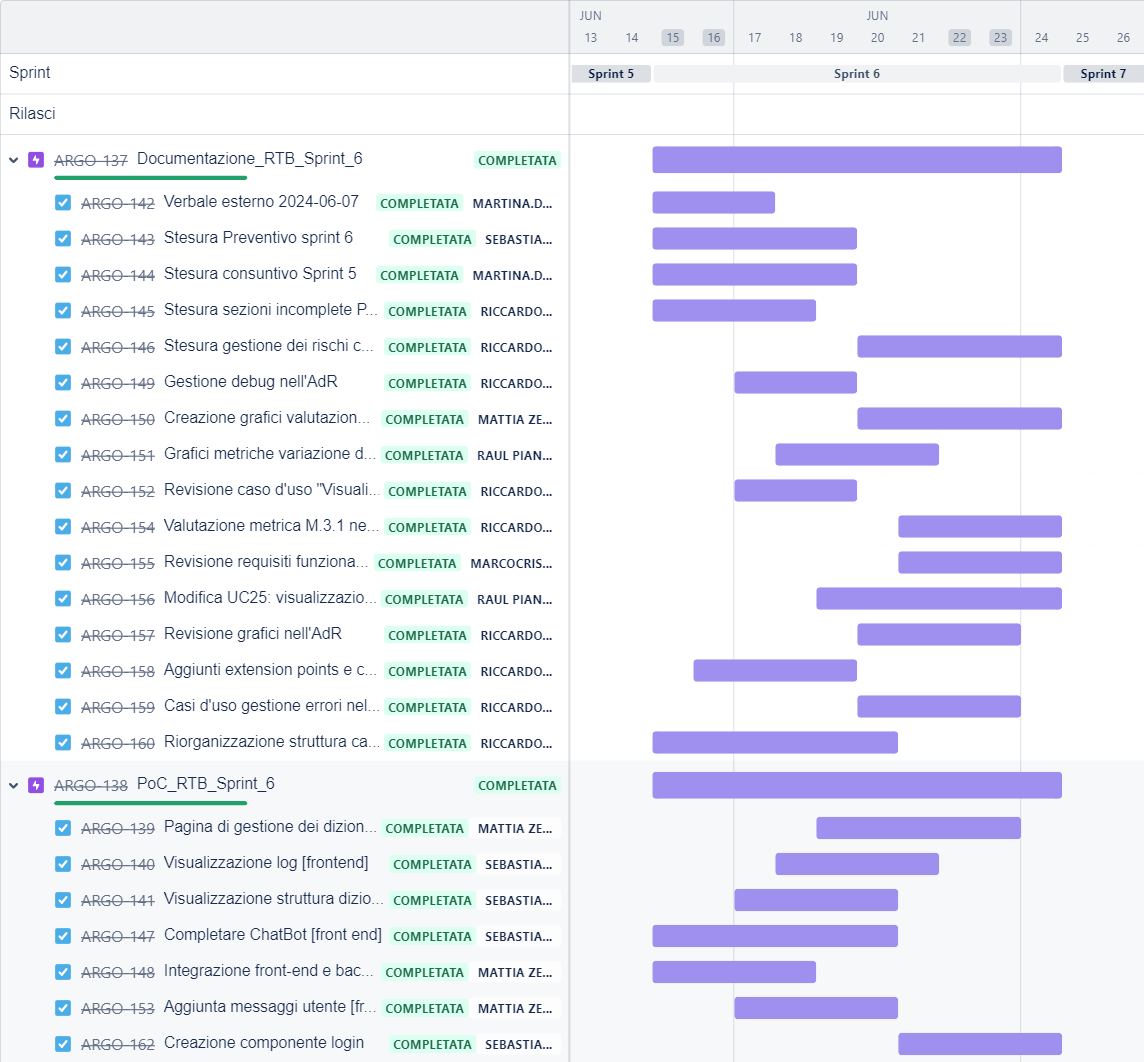
\includegraphics[width=0.90\textwidth]{assets/Pianificazione/Sprint-6/gantt.png}
  \caption{Sprint 6 - Diagramma di Gantt}\label{fig:sprint-6-gantt}
\end{figure}
